\chapter{Herramientas y tecnologías}
\label{chap:tecnoloxias}

\lettrine{E}{n} este capítulo, se describen las principales herramientas y tecnologías utilizadas durante el desarrollo de las prácticas. Se detallan tanto las herramientas de desarrollo como las tecnologías de Machine Learning y visión artificial empleadas.


\section{Herramientas de desarrollo}\label{sec:tecnologias}

\subsection{Control de versiones y gestión del código}\label{subsec:git}
Durante las prácticas se utilizó Git como sistema de control de versiones, junto con GitLab para el alojamiento de repositorios. Además, se emplearon las siguientes herramientas:

\begin{itemize}
    \item \textbf{pre-commit}: Herramienta\cite{pre_commit} que automatiza verificaciones en los repositorios, asegurando la unificación del formato del código y la generación de docstrings según convenciones definidas.
    \item \textbf{GitLab CI/CD}: Sistema\cite{gitlab_ci} de integración y despliegue continuo que permite ejecutar pipelines automatizados para pruebas, construcción y despliegue de aplicaciones.
    \item \textbf{DVC (Data Version Control)}: Herramienta\cite{dvc} para el versionado de datasets y modelos de Machine Learning, asegurando la reproducibilidad y rastreabilidad de experimentos.
\end{itemize}

\subsection{Entorno de desarrollo}\label{subsec:entorno}
El desarrollo se realizó principalmente en Python, utilizando:

\begin{itemize}
    \item \textbf{Visual Studio Code}: IDE\cite{vscode} principal utilizado para la escritura, depuración y administración del código con extensiones específicas para Python.
    \item \textbf{Docker y docker-compose}: Herramientas\cite{docker} para la contenerización, facilitando la creación de entornos aislados y reproducibles para el desarrollo y la ejecución de aplicaciones.
    \item \textbf{Conda y venv}: Utilizados\cite{conda}\cite{venv} para la gestión de entornos virtuales en Python, permitiendo un manejo eficiente de dependencias.
    \item \textbf{CMake y Make}: Herramientas\cite{cmake} empleadas para la configuración y compilación de proyectos, especialmente útiles en componentes de software de bajo nivel.
\end{itemize}

\section{Tecnologías de Machine Learning y Visión Artificial}
\label{sec:ml}

\subsection{MLflow}\label{subsec:mlflow}
Se utilizó MLflow\cite{mlflow} para la gestión de experimentos de Machine Learning, permitiendo:

\begin{itemize}
    \item \textbf{Tracking de métricas y parámetros}: Registro de datos relevantes durante los entrenamientos, como la pérdida y las tasas de aprendizaje.
    \item \textbf{Versionado de modelos}: Gestión de diferentes versiones de modelos entrenados, facilitando su comparación y reutilización.
    \item \textbf{Comparación de experimentos}: Análisis detallado entre distintas ejecuciones para identificar las configuraciones más efectivas.
    \item \textbf{Reproducibilidad de resultados}: Garantiza que los experimentos sean replicables al registrar todas las configuraciones necesarias.
\end{itemize}

\begin{figure}[hp!]
  \centering
  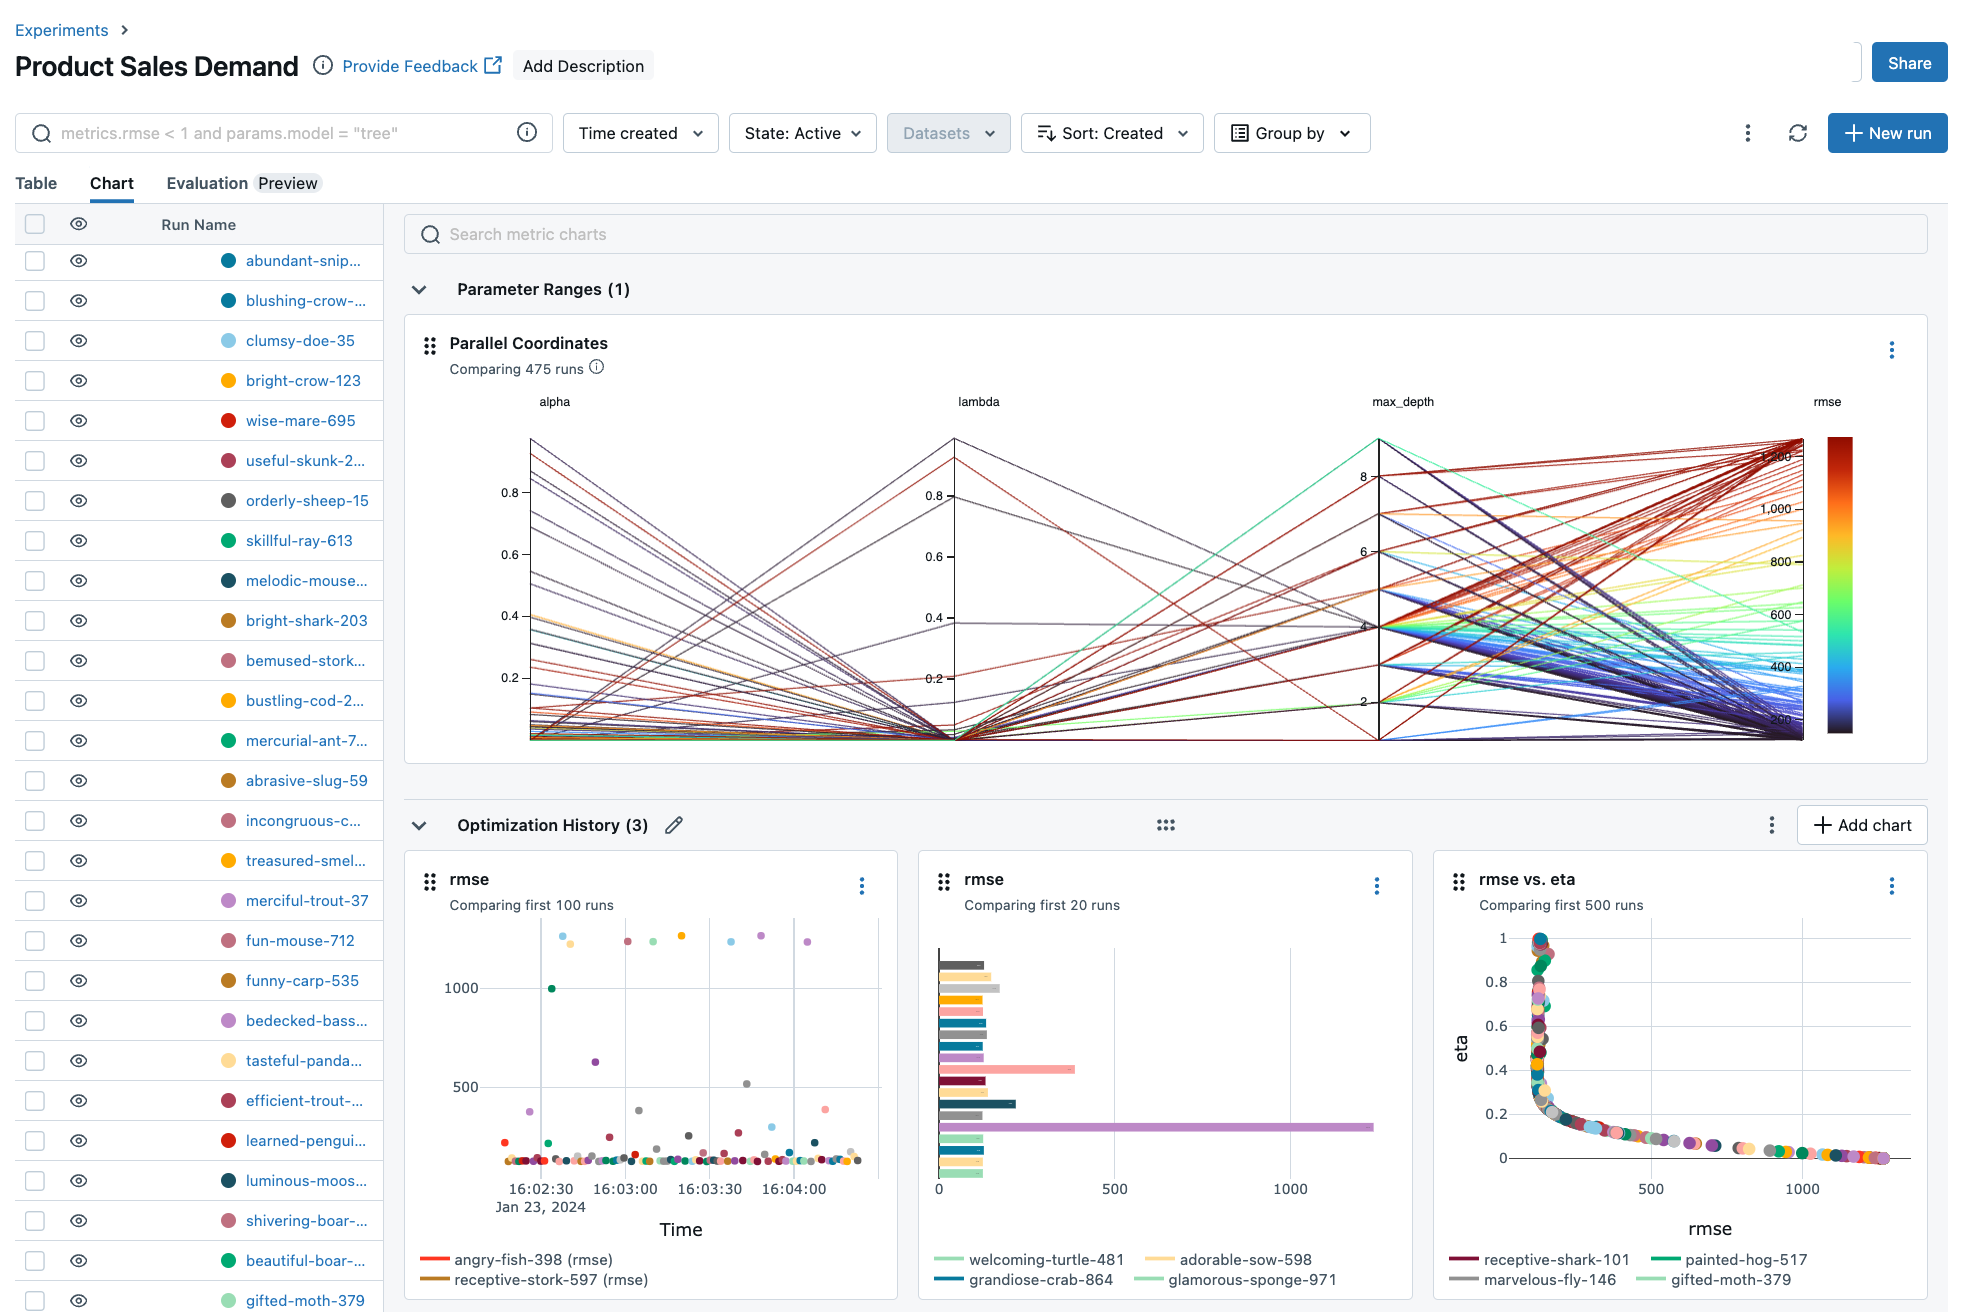
\includegraphics[width=0.8\textwidth]{04_imaxes/mlflow_example.png}
  \caption{Interfaz de gestión de experimentos en MLflow}
  \label{fig:mlflow}
\end{figure}

\subsection{CVAT}\label{subsec:cvat}
Para el etiquetado de datos se empleó CVAT\cite{cvat} (Computer Vision Annotation Tool), que permite:

\begin{itemize}
    \item \textbf{Etiquetado de videos frame a frame}: Ofrece una interfaz intuitiva para marcar objetos en cada fotograma.
    \item \textbf{Definición de bounding boxes}: Herramienta esencial para delimitar regiones de interés en imágenes o videos.
    \item \textbf{Exportación en múltiples formatos}: Compatible con una amplia variedad de formatos estándar en proyectos de visión artificial.
    \item \textbf{Trabajo colaborativo}: Facilita la asignación de tareas y la colaboración entre varios usuarios en un mismo proyecto.
\end{itemize}

\begin{figure}[hp!]
  \centering
  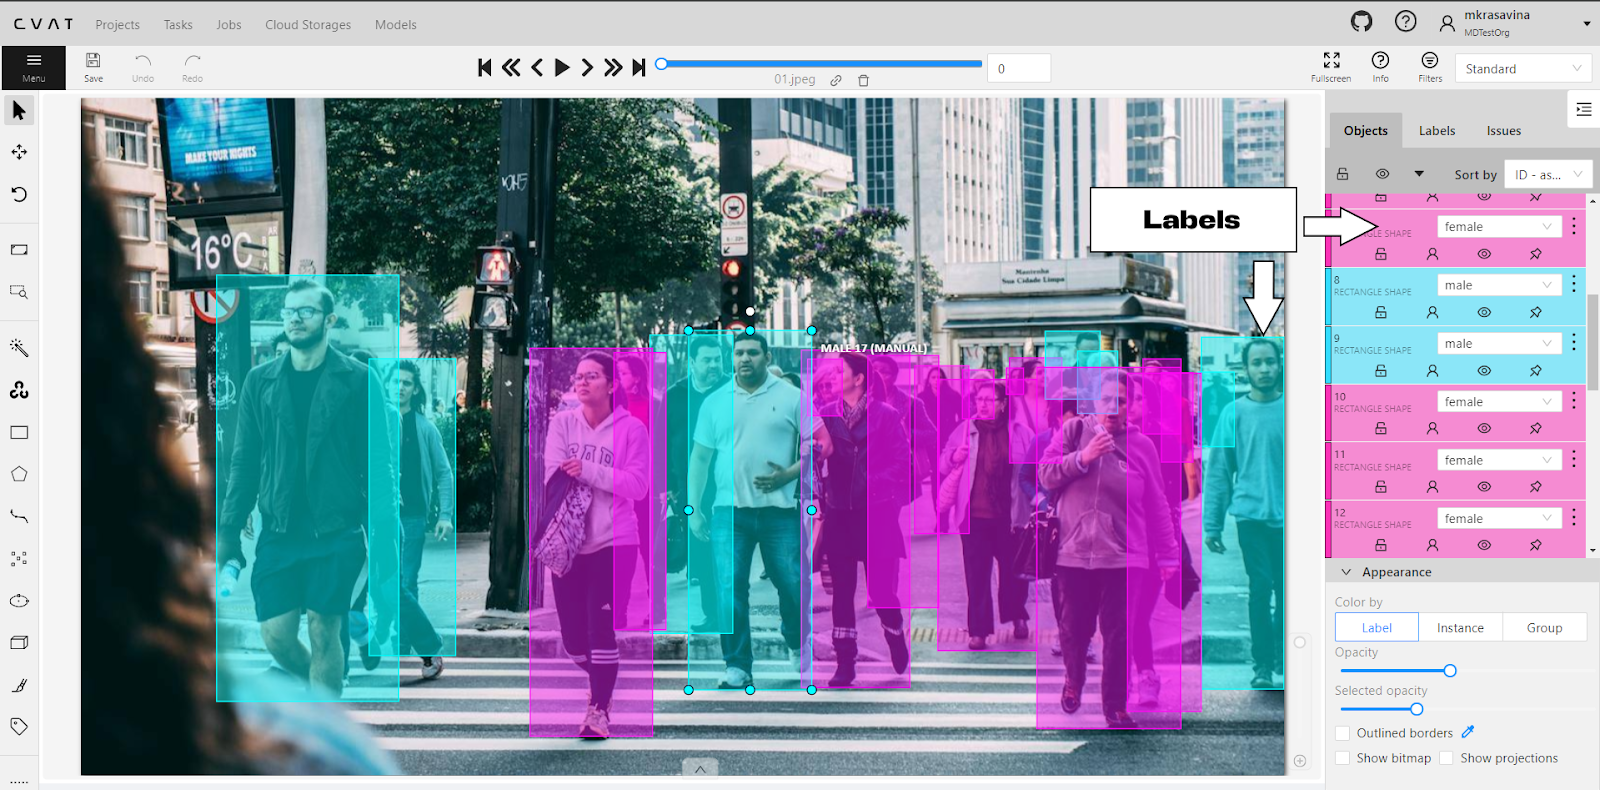
\includegraphics[width=0.8\textwidth]{04_imaxes/cvat_example.png}
  \caption{Ejemplo de etiquetado en CVAT}
  \label{fig:cvat}
\end{figure}

\section{Tecnologías de Síntesis de Voz (TTS)}
\label{sec:tts}

Durante las prácticas se evaluaron múltiples modelos de Text-to-Speech (TTS), analizando sus características y capacidades. A continuación, se presentan los modelos evaluados:

\subsection{Coqui TTS}\label{subsec:coqui}
Plataforma\cite{coqui_tts} de código abierto que incluye múltiples modelos TTS:
\begin{itemize}
    \item \textbf{XTTSv2}: Especializado en clonación de voz, permitiendo la reproducción de voces específicas con alta fidelidad.
    \item \textbf{Tacotron2 con HiFi-GAN}: Combinación\cite{tacotron2} de un modelo de texto a mel-espectrograma (Tacotron2) con un generador de audio de alta calidad (HiFi-GAN), ideal para síntesis natural.
    \item \textbf{VITS}: Modelo\cite{vits} integrado para síntesis de voz y conversión de voz a texto, que equilibra calidad y rapidez.
\end{itemize}

\subsection{IMS-Toucan}\label{subsec:ims_toucan}
Modelo\cite{ims_toucan} de síntesis desarrollado por el Instituto de Ciencias de la Computación de Stuttgart. Ofrece capacidades avanzadas de generación de voz con enfoque en la naturalidad y entonación, aunque no incluye soporte completo para clonación de voz. Dispone de cierta compatibilidad con clonación de voz pero, la voz generada, será como la voz más similar empleada en el entrenamiento. Sin embargo, esto puede mitigarse en parte mediante el fine-tunning.

\subsection{Otros modelos evaluados}\label{subsec:other_models}
Además de los anteriores, se probaron los siguientes modelos TTS:

\begin{itemize}
    \item \textbf{OpenVoice v2}: Sistema\cite{openvoice} TTS flexible y de código abierto, diseñado para personalización y soporte multilingüe.
    \item \textbf{Real-Time-Voice-Cloning}: Modelo que combina Tacotron y redes neuronales para realizar clonación de voz y síntesis de alta calidad en tiempo real.
    \item \textbf{Mozilla TTS}: Plataforma\cite{mozilla_tts} modular y extensible para la síntesis de voz, enfocada en facilitar la creación de modelos personalizados y adaptativos.
\end{itemize}

\subsection{Modelos que no soportan clonado de voz}\label{subsec:no_clonado}

A lo largo de las prácticas se evaluaron diversos modelos de Text-to-Speech que no cuentan con capacidad de clonación de voz. A continuación, se listan algunos de ellos:

\begin{itemize}
    \item \textbf{eSpeak}: Motor TTS ligero y rápido que genera síntesis de voz basada en reglas. Aunque no soporta clonado, es eficiente para dispositivos de baja capacidad.
    \item \textbf{Festival}: Sistema TTS modular y flexible que ofrece varias opciones para la generación de voces sintéticas, pero carece de funcionalidad para clonación.
    \item \textbf{Mimic1}: Derivado de Festival, Mimic1 permite una síntesis rápida con diferentes voces preconfiguradas, sin soporte para clonación de voz.
    \item \textbf{Mimic3}: Continuación de Mimic1, diseñada para síntesis offline con menor latencia y mejor calidad de audio, pero sin capacidades de clonación.
    \item \textbf{Pico TTS}: Solución compacta para la síntesis de texto a voz orientada a dispositivos móviles, sin características avanzadas como la clonación.
    \item \textbf{Flite}: Variante ligera de Festival que se utiliza en sistemas embebidos para tareas de síntesis básica de voz.
    \item \textbf{Mary TTS}: Plataforma extensible para la síntesis de voz que soporta múltiples idiomas y configuraciones, pero no incluye clonado.
    \item \textbf{Piper}: Modelo optimizado para la generación rápida de audio TTS con una calidad aceptable, aunque no soporta clonación.
    \item \textbf{FastSpeech 2}: Modelo TTS basado en arquitectura Transformer que ofrece síntesis eficiente, pero sin capacidades de clonado directo.
    \item \textbf{TransformerTTS}: Sistema TTS basado en Transformers que produce voces naturales pero no admite clonación.
    \item \textbf{Tensorflow TTS}: Conjunto de modelos TTS basados en TensorFlow que incluyen varias arquitecturas avanzadas, sin funcionalidad de clonado.
    \item \textbf{PaddleSpeech}: Biblioteca TTS de código abierto que soporta múltiples modelos, enfocada en la síntesis pero sin capacidades de clonación.
    \item \textbf{Glow Speak}: Basado en la arquitectura Glow, este modelo TTS permite una síntesis precisa pero no incluye soporte para clonado de voz.
\end{itemize}

\section{Otras herramientas}
\label{sec:otras}

\begin{itemize}
    \item \textbf{ffmpeg}: Para procesamiento de video y audio\\
        Es una solución\cite{ffmpeg} multiplataforma ampliamente utilizada para la grabación, conversión y transmisión de archivos de audio y video. En este proyecto, se empleó para tareas como el recorte de videos/audios y la conversión de formatos, lo que permitió optimizar recursos (wav >> mp3) y garantizar compatibilidad con diferentes plataformas. 
    \item \textbf{VIA} (VGG Image Annotator): Para etiquetado de imágenes\\
        Una herramienta\cite{via} ligera y sencilla para el etiquetado de imágenes. Es crucial para preparar conjuntos de datos, ya que permite definir áreas de interés en imágenes (bounding boxes, máscaras, etc.) y asignarles etiquetas personalizadas. En este proyecto, se utilizó para generar anotaciones necesarias para entrenar modelos de reconocimiento de dígitos en marcadores.
        \begin{figure}[hp!]
          \centering
          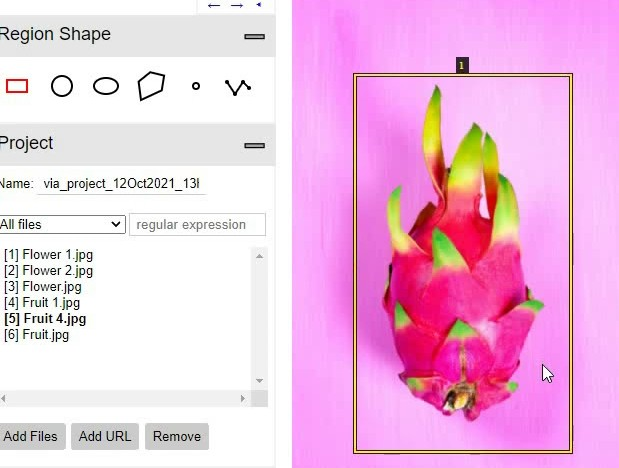
\includegraphics[width=0.8\textwidth]{04_imaxes/via_example.jpg}
          \caption{Ejemplo de etiquetado en VIA}
          \label{fig:via}
        \end{figure}
    \item \textbf{Whisper}: Para transcripción de audio\\
        Una solución desarrollada por OpenAI para la transcripción automática de audio en texto. Es una herramienta\cite{whisper} robusta que admite múltiples idiomas y ofrece transcripciones con alta precisión incluso en condiciones de ruido. Su utilización fue clave para procesar grabaciones de audio y convertirlas en datos textuales que posteriormente fueron empleados para la generación de los datasets utilizados para realizar el fine-tunning de modelos TTS.
    \item \textbf{JIRA}: Para gestión de tareas y tickets\\
        Es una plataforma\cite{jira} de gestión de tareas y seguimiento de tickets ampliamente adoptada en entornos de desarrollo de software y gestión de proyectos. La emplea la empresa para organizar y priorizar tareas, registrar incidencias, y facilitar la colaboración entre los diferentes miembros del equipo. Su capacidad para generar informes y estadísticas también contribuye al seguimiento del progreso de los proyectos y a la toma de decisiones basada en datos.\\
        En mi caso, se me asignaron trabajos o incidencias a resolver mediante dicha plataforma.
    \item \textbf{Demucs}: Para la limpieza de audios.\\
        Es un modelo\cite{demucs} de aprendizaje profundo diseñado para la separación de fuentes de audio. Permite dividir una pista de audio en componentes como voz, instrumentos y ruido de fondo, lo que facilita la limpieza y mejora de grabaciones. En este proyecto, se utilizó para aislar el contenido relevante de grabaciones de audio, eliminando ruidos no deseados y mejorando la calidad de las pistas procesadas, que serían empleadas en el para generar los datasets junto con Whisper.
     \item \textbf{OpenCV}: Para procesamiento de imágenes y visión por computadora.\\
        Es una biblioteca\cite{opencv} de código abierto ampliamente utilizada para tareas de visión artificial. Incluye funciones avanzadas para manipulación de imágenes, detección de objetos, reconocimiento facial, y análisis de video. En este proyecto, se utilizó para representar las interfaces gráficas de las utilidades, así como para interactuar con las imágenes mostradas.
    \item \textbf{Tkinter}: Para la creación de interfaces gráficas de usuario (GUI).\\
        Biblioteca estándar de Python para el desarrollo de interfaces gráficas. Proporciona herramientas para crear ventanas, botones, cuadros de texto, y otros componentes interactivos. En este proyecto, se utilizó para desarrollar una interfaz intuitiva que facilitara la interacción con el usuario, permitiendo configurar marcadores de forma sencilla, sin necesidad de realizar cambios manualmente en los json.

\end{itemize}